\documentclass[letterpaper, 9pt, conference]{ieeeconf}  % Comment this line out if you need a4paper
%\documentclass[a4paper, 10pt, conference]{ieeeconf}      % Use this line for a4 paper
\IEEEoverridecommandlockouts                              % This command is only needed if 
                                                          % you want to use the \thanks command

\overrideIEEEmargins                                      % Needed to meet printer requirements.

% See the \addtolength command later in the file to balance the column lengths
% on the last page of the document

% The following packages can be found on http:\\www.ctan.org
%\usepackage{graphics} % for pdf, bitmapped graphics files
%\usepackage{epsfig} % for postscript graphics files
%\usepackage{mathptmx} % assumes new font selection scheme installed
%\usepackage{times} % assumes new font selection scheme installed
%\usepackage{amsmath} % assumes amsmath package installed
%\usepackage{amssymb}  % assumes amsmath package installed


\usepackage{times}
%\usepackage{natbib}
\usepackage{graphicx}
\usepackage{fixme} % This package provides a way to insert notes in draft documents
\usepackage{amsmath}
%\usepackage{multicols}
\usepackage{adjmulticol}
\usepackage{subfig}
\usepackage{url}
\usepackage{cite}

%\usepackage[]{algorithm2e}
%\usepackage[]{algorithmic}


\title{\LARGE \bf
%Preparation of Papers for IEEE Sponsored Conferences \& Symposia*
Optimal Sample Based Manipulator Motion Planning}


\author{Behnam Asadi$^{1}$ 
\thanks{$^{1}$Behnam Asadi is a researcher at mathematics and computer science department of university of Bremen, Germany.
        {\tt\small behnam.asadi@gmail.com}}%
\thanks{This work was supported through two grants of the German Federal Ministry of Economics and Technology (BMWi, FKZ 50 RA 1216 and FKZ 50 RA 1217 ).}
}
\begin{document}



\maketitle
\thispagestyle{empty}
\pagestyle{empty}




\begin{abstract}

bla blah
\end{abstract}
Keywords: Manipulator motion planning, dual arm operation, planning under Cartesian constraint, robotics. 

%%%%%%%%%%%%%%%%%%%%%%%%%%%%%%%%%%%%%%%%%%%%%%%%%%%%%%%%%%%%%%%%%%%%%%%%%%%%%%%%
\section{INTRODUCTION}\label{Introduction}

\section{RRT Star}\label{RRT_Star}




Sample based algorithms for motion such as RRT and PRM planning are very robust in finding a solution even in space with high dimensionality or environment occluded with obstacles with guarantees of probabilistic completeness. One main drawback of these algorithm is the lack of quality of the solution.
Generated trajectories from sample based motion planner are usually jerky, seems unnatural and might have redundant movements.
PRM∗ and RRT∗ are two algorithms based on sample based algorithm but have the capability of optimizing the solution. The algorithm asymptotically optimal, such that the solution almost surely converges to the optimum \cite{karaman2011sampling}.

 Moreover, it is shown that the computational complexity of the new algorithms is within a constant factor of that of their probabilistically complete (but not asymptotically optimal) counterparts. The analysis in this paper hinges on novel connections between stochastic sampling-based path planning algorithms and the theory of random geometric graphs.

















\section{EDT}\label{EDT}



The \textbf{dynamicEDT3D} library \cite{dynamicEDT3D} provides EDT (Euclidean distance transform) map in 3D. 
The library can hook into an  OctoMap \cite{wurm2010octomap} and detect the changes to update the map efficiently rather than computing the map from scratch.


The return value form collision detection tools such as FCL \cite{pan2012fcl} determines the state of collisions/ non collision  and the optimizer algorithm can not learn the distances for all body part of the robot from the environment.


%checking the optimizer can not find the find the optimal path
%due to the which returns only collision/ no collision  can not properly find the optimal path while if we provide the optimiser with information in each state (i.e the sum of distances to the closest obstacle) the solution will lead to optimal path
%Here in this work we created an OctoMap from the obstacles in the environment and fed it to  dynamicEDT3D. Later we used this map to find 
%
%We also modelled the collision tag of robot model in URDF with series of spheres. Since the sphere has no orientation, by knowing the center  of sphere and the radius and having EDT map, the distance to the closest obstacle could be determined. 
%The motivation is 
%
%
%
%
%
%When applying CHOMP, we typically use a simplified
%geometric description of our robots, approximating the robot
%as a “skeleton” of spheres and capsules, or line-segment
%swept spheres. For a sphere of radius r with center x, the
%distance from any point in the sphere to the nearest obstacle
%is no less than d(x) − r. An analogous lower bound holds
%for capsules.
%There are a few key advantages of using the signed
%distance field to check for collisions. Collision checking is
%very fast, taking time proportional to the number of voxels
%occupied by the robot’s “skeleton”. Since the signed distance
%field is stored over the workspace, computing its gradient via
%finite differencing is a trivial operation. Finally, because we
%have distance information everywhere, not just outside of
%obstacles, we can generate a valid gradient even when the
%robot is in collision – a particularly difficult feat for other
%representations and distance query methods.




\section{Optimal Path Planning}\label{Optimal_Path_Planning}
In this example we have the various objective function including path minimization, obstacle avoidance(maximum clearance)
and combination of both have been examined









\paragraph{Optimal Planning}
One of the drawbacks of sample based planners is that the computed path doesn't look natural and no optimisation has been done on the path. In this work I have 
worked on sample based optimization planners which have robustness of sample based planner and the capability of adding objective function.
Different objective functions have been investigated including: minimizing the path length, maximizing clearance or combination of both.
Figure \ref{sample_based_optimization_based_problem2} illustrates an example of employing different objective function and the generated path.

Figure \ref{sample_based_optimization_based_problem2}(a) define the problem, white area is the free space, black bar is the obstacle and the red dots are start and goal. Figure \ref{sample_based_optimization_based_problem2}(b) is the euclidean distance map of the problem. The area with darker gray are closer to the closest obstacle. In Figure \ref{sample_based_optimization_based_problem2}(c), the planner tries to find path between start and goal pose while maximizing the clearance.
In Figure \ref{sample_based_optimization_based_problem2}(d), the objective function is path minimizations and the planner find the shortest path. In Figure \ref{sample_based_optimization_based_problem2}(e) and (f) we employed a combination of both  objective function with different weights 








\begin{figure*}
\centering
\subfloat[]
{
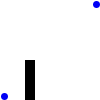
\includegraphics[width=0.30\textwidth]{figures/AP4300/problem2/problem.png}
}
\subfloat[]
{
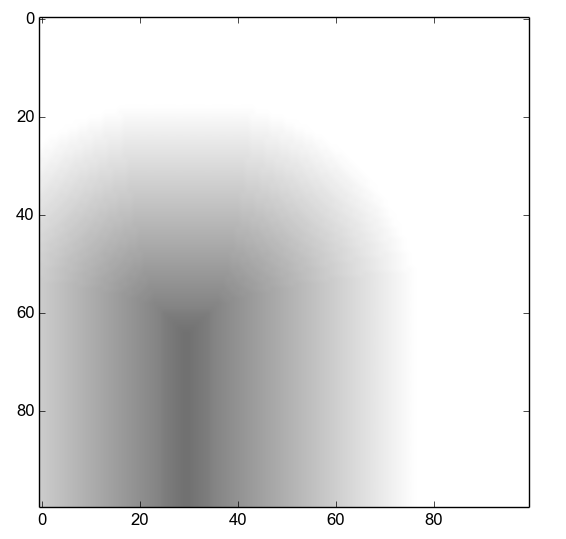
\includegraphics[width=0.30\textwidth]{figures/AP4300/problem2/edt.png}
}
\subfloat[]
{
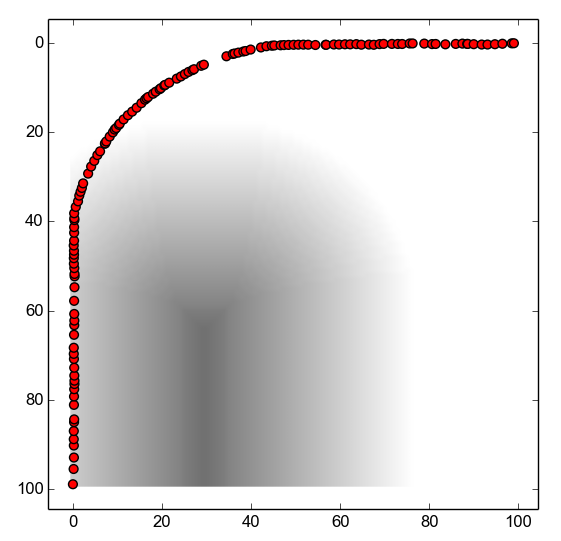
\includegraphics[width=0.30\textwidth]{figures/AP4300/problem2/getClearanceObjective.png}
}


\subfloat[]
{
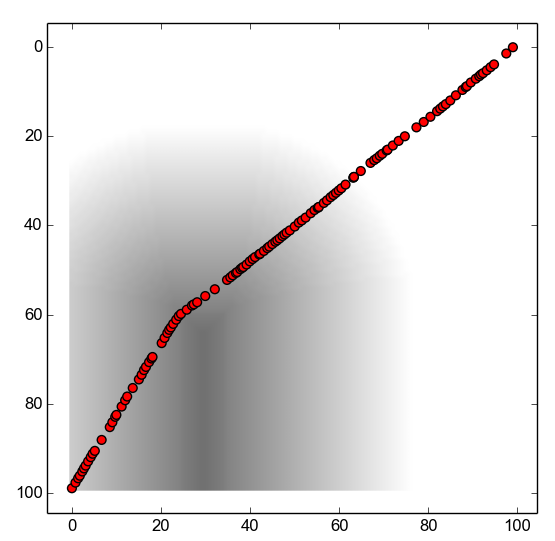
\includegraphics[width=0.30\textwidth]{figures/AP4300/problem2/getPathLengthObjective.png}
}
\subfloat[]
{
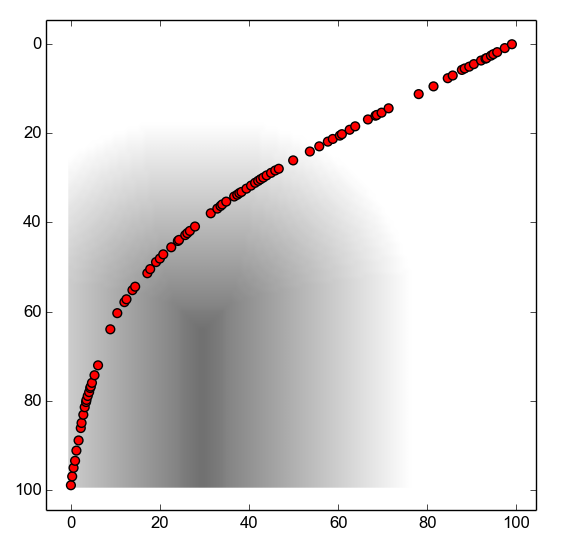
\includegraphics[width=0.30\textwidth]{figures/AP4300/problem2/getBalancedObjective1_length_1_clearance_5.png}
}
\subfloat[]
{
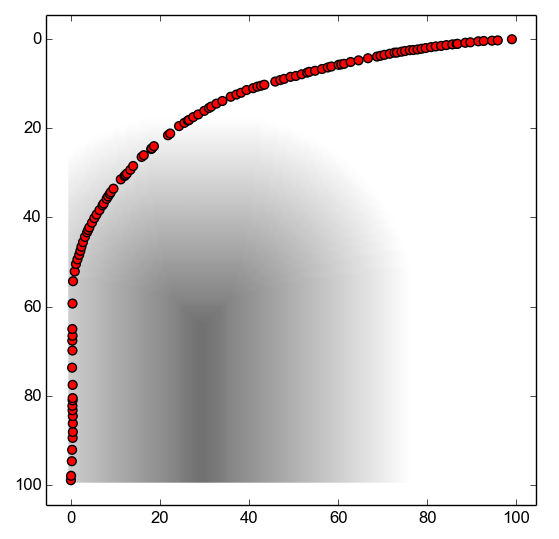
\includegraphics[width=0.30\textwidth]{figures/AP4300/problem2/getBalancedObjective_length_1_clearance_50.png}
}
\caption{Solving a motion planning problem by creating euclidean distance map from the environment and employing different objective function. The start and goal have meen marked by blue, the obstacle marked by black.}
\label{sample_based_optimization_based_problem1}
\end{figure*}


This concept has been extended into 3D space. The integration of code for manipulator motion planning is still under progress.













\begin{figure*}
\centering
\subfloat[]
{
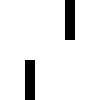
\includegraphics[width=0.30\textwidth]{/home/behnam/Asadi/OptimalPlanningWithRRT/figures/problem.png}
}
\subfloat[]
{
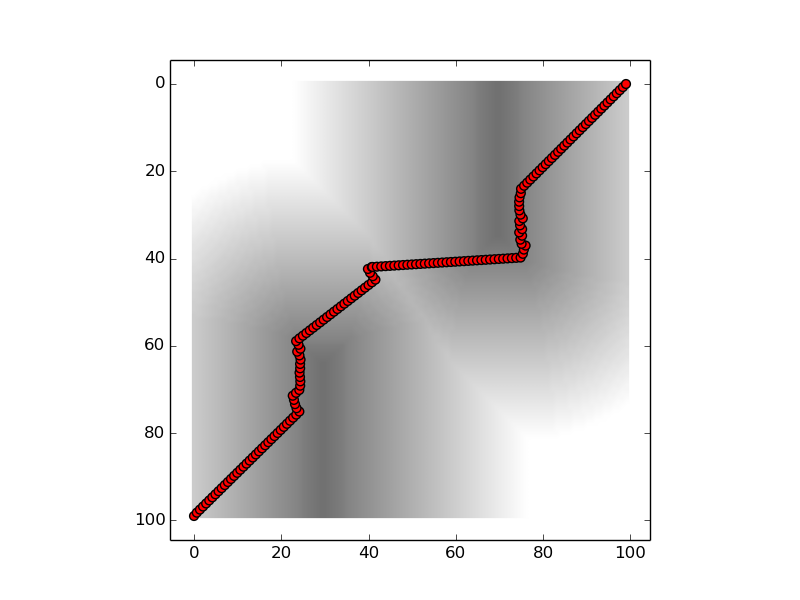
\includegraphics[width=0.30\textwidth]{/home/behnam/Asadi/OptimalPlanningWithRRT/figures/1.png}
}


\subfloat[]
{
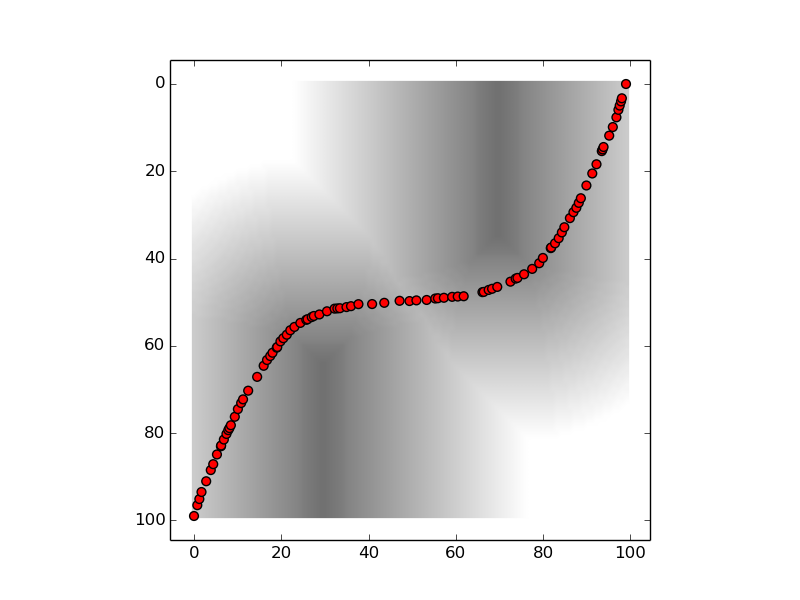
\includegraphics[width=0.30\textwidth]{/home/behnam/Asadi/OptimalPlanningWithRRT/figures/2.png}
}
\subfloat[]
{
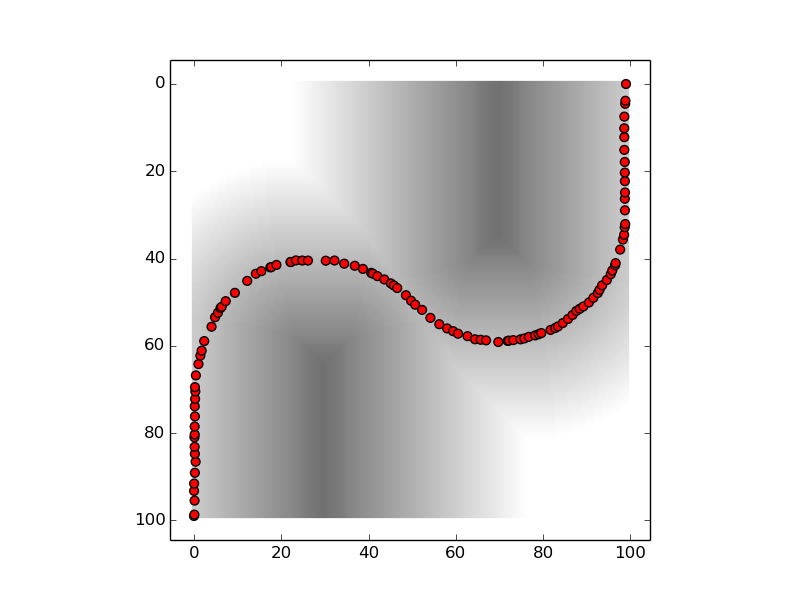
\includegraphics[width=0.30\textwidth]{/home/behnam/Asadi/OptimalPlanningWithRRT/figures/getClearanceObjective.png}
}
\caption{Solving a motion planning problem by creating euclidean distance map from the environment and employing different objective function.}
\label{sample_based_optimization_based_problem2}
\end{figure*}










\section{Optimal Manipulator Motion Planning}\label{Optimal_Manipulator_Motion_Planning}

\section{Analysis and Conclusion}






\bibliographystyle{ieeetr}
%\bibliographystyle{abbrv}
%\bibliographystyle{unsrtnat}
\bibliography{references}{}

\end{document}